\chapter{Відкриті дані в Україні}

\subsection{Законодавство України щодо відкритих даних та готовність країни до впровадження}

\begin{enumerate}
    \item \href{http://zakon2.rada.gov.ua/laws/show/319-19}{Положення про набори даних, які підлягають оприлюдненню у формі відкритих даних № 835 (редакція від 21.10.2015)}
    \item \href{https://drive.google.com/file/d/0B1kGsKt9XV_QaFZVaTZiT19aRTA/view}{План заходів (дорожня карта) розвитку відкритих даних на 2016 рік}
    \item Єдиний державний портал відкритих даних \href{https://data.gov.ua/}{data.gov.ua — Керівництво користувача}
    \item Єдиний державний портал відкритих даних \href{https://data.gov.ua/}{data.gov.ua — Робота з API}
    \item \href{https://docs.google.com/document/d/1g5VUhUzjgTVvcp7zvlWbCUsmoJNaQ6w4T3vacYSu34U/edit}{Open Data Readiness Assessment (ODRA) Ukraine Final Report}
\end{enumerate}

\subsection{Україна у світових рейтингах}

\subsubsection{Open Data Barometer}

\begin{itemize}
    \item Сайт: \href{http://www.opendataresearch.org/barometer}{opendataresearch.org/barometer}
\end{itemize}

Open Data Barometer — спільний дослідницький проєкт Open Data Institute та World Wide Web Foundation. Аналізує глобальні тенденції розвитку відкритих даних, надає порівняльні дані по країнах і регіонах. Україна займає 62 місце із 86 проаналізованих країн (2015 — 55 місце).

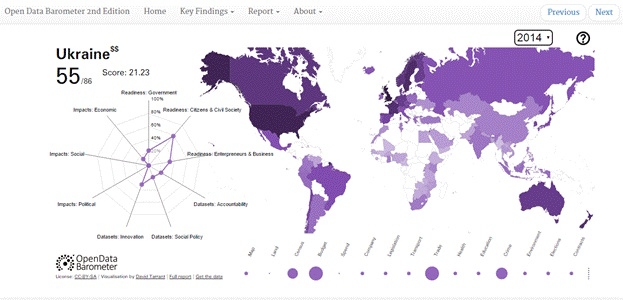
\includegraphics{images/010.gif}
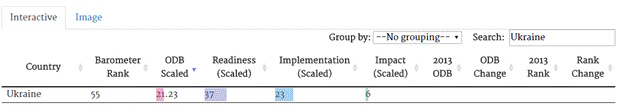
\includegraphics{images/011.gif}
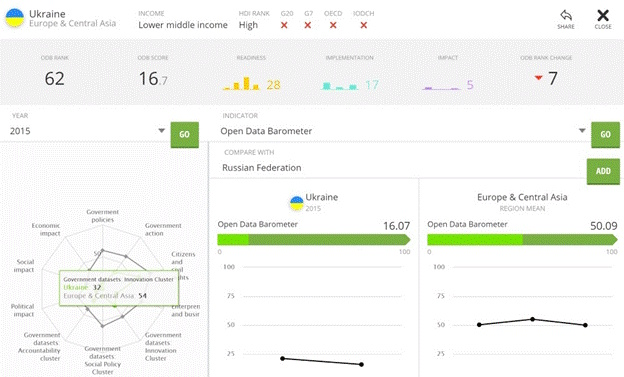
\includegraphics{images/012.gif}

\subsubsection{Open Data Index}

\begin{itemize}
    \item Сайт: \href{https://index.okfn.org/}{index.okfn.org}
\end{itemize}

Масштабний дослідницький проєкт Open Knowledge Foundation щодо відкритості державних даних у світі. Україна — 54 місце у глобальному рейтингу (2015 рік).

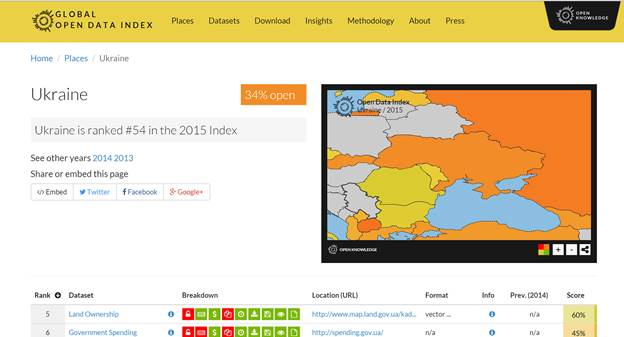
\includegraphics{images/013.jpg}

\subsubsection{The Web Index}

\begin{itemize}
    \item Сайт: \href{http://thewebindex.org/}{thewebindex.org}
\end{itemize}

Рейтинг розвитку інтернету в країнах світу від World Wide Web Foundation. Україна — 46 місце серед 86 країн.

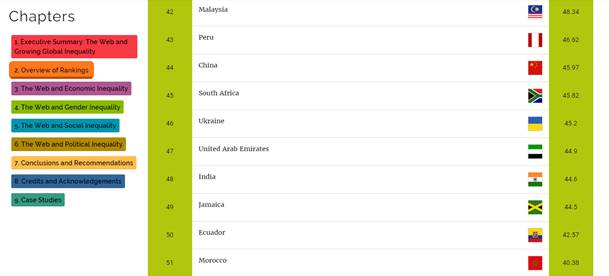
\includegraphics{images/014.jpg}

\subsubsection{Open Budget Survey}

\begin{itemize}
    \item Сайт: \href{http://internationalbudget.org/what-we-do/open-budget-survey/}{internationalbudget.org/what-we-do/open-budget-survey/}
\end{itemize}

Рейтинг відкритості державних бюджетів від International Budget Partnership. Оцінки для України:
\begin{itemize}
    \item Прозорість (відкритий бюджет): 46/100
    \item Участь громадськості: 23/100
    \item Нагляд державним органом: 79/100
    \item Нагляд вищого органу фінансового контролю: 83/100
\end{itemize}

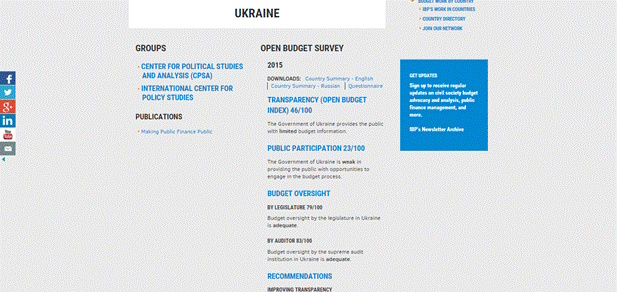
\includegraphics{images/015.gif}

\subsubsection{E-Government for the People}

\begin{itemize}
    \item Сайт: \href{http://www.unpan.org/egovkb/global_reports/08report.html}{unpan.org/egovkb/global_reports/08report.html}
\end{itemize}

Рейтинг ООН з розвитку електронного уряду. Коефіцієнт розвитку електронного уряду України — між 0,5 та 0,75.

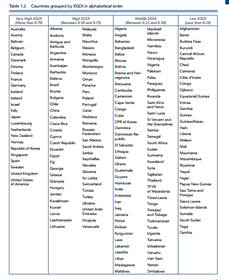
\includegraphics{images/016.jpg}

\subsection{Проєкти на базі відкритих даних}

\subsubsection{Нові назви вулиць, площ Дніпропетровська}

\begin{itemize}
    \item \href{http://rename.dp.ua/}{rename.dp.ua} — повний перелік нових назв вулиць і площ Дніпропетровська.
\end{itemize}


\includegraphics{images/017.gif}

\subsubsection{ДонорUA}

\begin{itemize}
    \item \href{http://donor.ua/}{donor.ua} — координація донорів крові та пропаганда донорства в Україні.
\end{itemize}

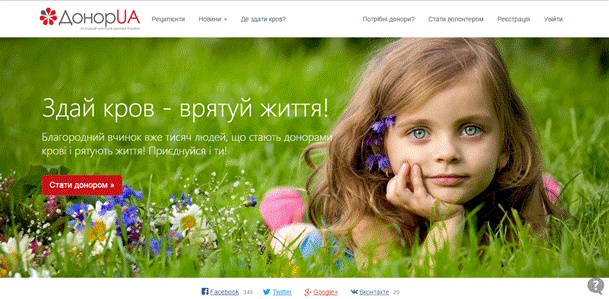
\includegraphics{images/018.gif}

\subsubsection{УкрТрансГаз}

\begin{itemize}
    \item \href{http://utg.ua/live/}{utg.ua/live/} — карта трубопроводів, сховищ та обсягів газу.
\end{itemize}

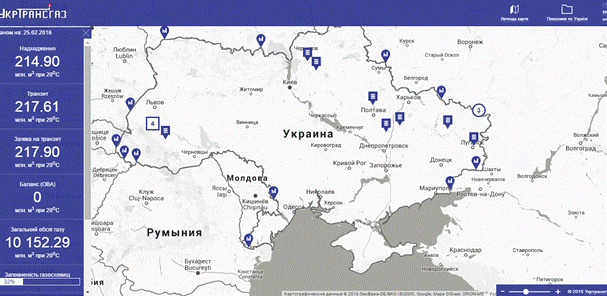
\includegraphics{images/019.gif}

\subsubsection{НБУ}

\begin{itemize}
    \item \href{http://nbu.rocks/}{nbu.rocks} — відкриті дані Національного Банку України про банки.
\end{itemize}

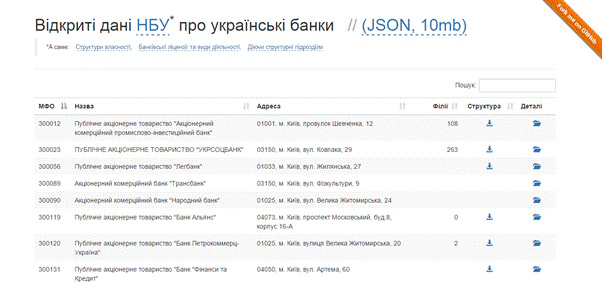
\includegraphics{images/020.gif}

\subsubsection{3G.Multitest.ua}

\begin{itemize}
    \item \href{http://3g.multitest.ua/}{3g.multitest.ua} — карта покриття 3G GSM операторів України.
\end{itemize}

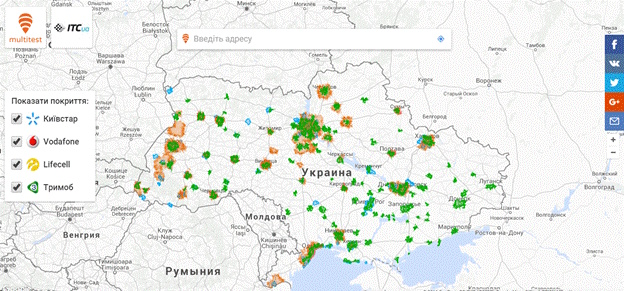
\includegraphics{images/021.gif}

\subsubsection{Агенти змін}

\begin{itemize}
    \item \href{https://medium.com/@agentyzmin}{medium.com/@agentyzmin} — система орієнтування в Києві.
\end{itemize}

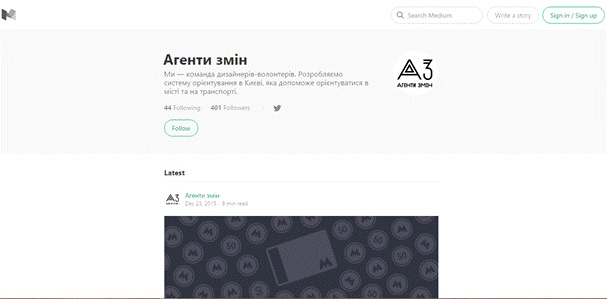
\includegraphics{images/022.gif}

\subsubsection{Лун.UA}

\begin{itemize}
    \item \href{http://www.lun.ua/}{lun.ua} — оренда та продаж нерухомості у Києві та Україні.
\end{itemize}

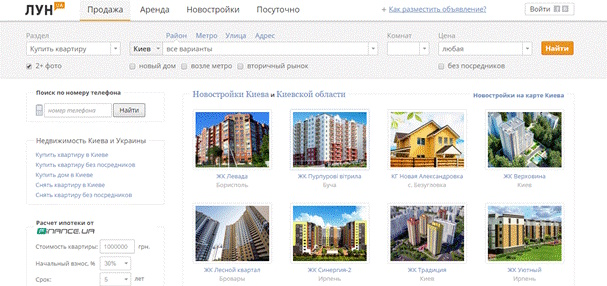
\includegraphics{images/023.gif}

\subsubsection{PEP.ORG.UA}

\begin{itemize}
    \item \href{http://pep.org.ua/uk/}{pep.org.ua/uk/} — відкритий реєстр національних публічних діячів України.
\end{itemize}

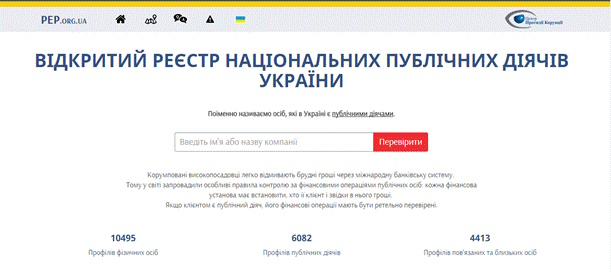
\includegraphics{images/024.gif}

\subsubsection{Посіпаки}

\begin{itemize}
    \item \href{http://posipaky.info/}{posipaky.info} — база даних помічників народних депутатів України.
\end{itemize}

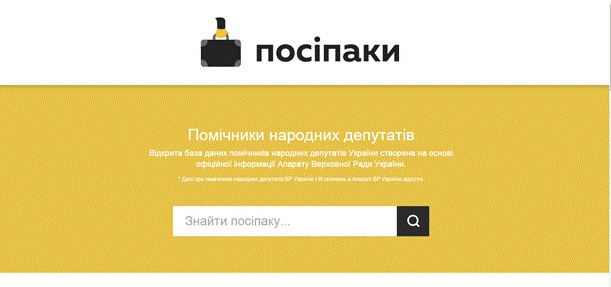
\includegraphics{images/025.gif}

\subsubsection{CityScale}

\begin{itemize}
    \item \href{http://www.cityscale.com.ua/}{cityscale.com.ua} — портал з інтерактивними картами умов життя.
\end{itemize}

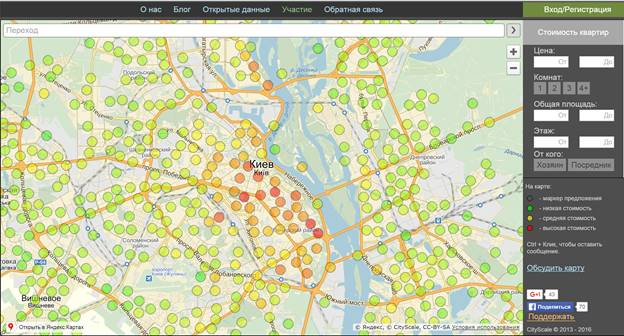
\includegraphics{images/026.jpg}

\subsubsection{ARBUZ}

Мобільний додаток для підвищення безпеки у містах на основі офіційних даних поліції.

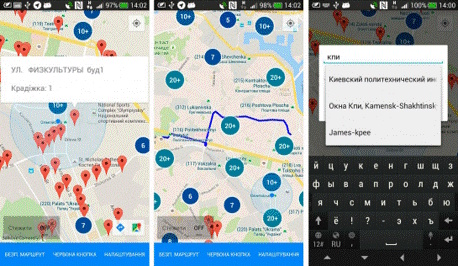
\includegraphics{images/027.gif}

\subsubsection{KyivSmartCity}

\begin{itemize}
    \item \href{http://re.kievcity.gov.ua/#/objects}{re.kievcity.gov.ua/#/objects} — система управління майном громади Києва.
\end{itemize}

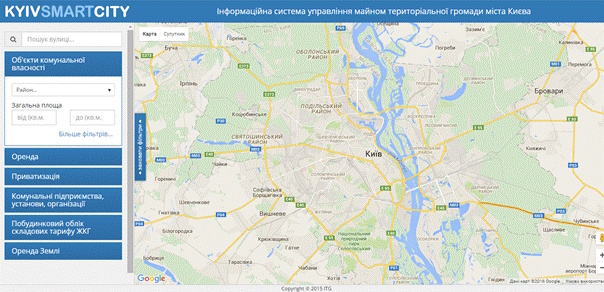
\includegraphics{images/028.gif}

\subsubsection{Видані направлення авіакомпаніям України}

\begin{itemize}
    \item \href{https://www.google.com/maps/d/viewer?mid=zQyzchol-IlQ.kqJvVjvXIY-s&hl=en_US}{Google Maps} — призначення для експлуатації міжнародних повітряних ліній.
\end{itemize}

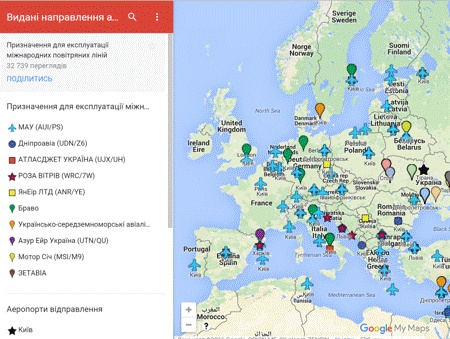
\includegraphics{images/029.gif}

\subsubsection{Tesla Club Ukraine}

\begin{itemize}
    \item \href{http://tesla-club.com.ua/gmap}{tesla-club.com.ua/gmap} — мережа заправок для електромобілів.
\end{itemize}

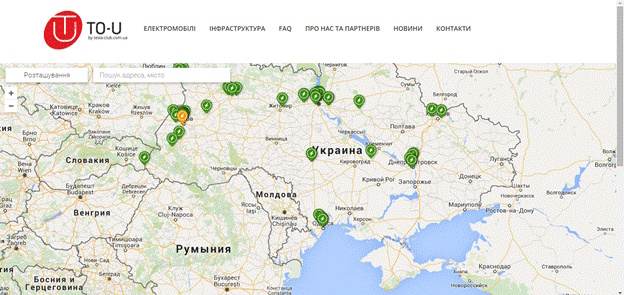
\includegraphics{images/030.gif}

\subsubsection{Дороги України}

\begin{itemize}
    \item \href{http://uaroads.com/}{uaroads.com} — інформація про стан доріг в Україні.
\end{itemize}

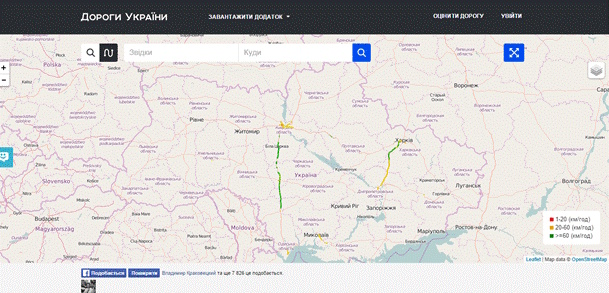
\includegraphics{images/031.gif}

\subsubsection{Інші проєкти}

\begin{enumerate}
    \item \href{http://data.rada.gov.ua/open/main/apps}{Додатки та сервіси на базі відкритих даних ВРУ}
    \item \href{http://opendata.rada.gov.ua/}{Портал відкритих даних ВРУ}
    \item \href{http://rada4you.org}{Як голосують депутати}
    \item Мобільний додаток «Zakonoproekt» для відстеження законопроєктів
    \item \href{http://knopkodavy.chesno.org/}{Кнопкодави}
    \item \href{http://groups.chesno.org/}{Візуалізація даних спільного ініціювання законопроєктів}
    \item \href{https://rada.oporaua.org/map/}{Приймальні депутатів}, \href{https://pryjmalni.chesno.org}{pryjmalni.chesno.org}
    \item \href{http://openvote.in.ua/}{Виборча варта}
    \item \href{https://e-vybory.org/}{Електронні вибори}
\end{enumerate}

\subsubsection{Інкубатор на базі відкритих даних 1991}

1991 — перший в Україні некомерційний інкубатор, що допомагає перетворити відкриті державні дані на стартапи для громадян, бізнесу та держави.

Програми інкубатора:
\begin{itemize}
    \item Галузеві рішення (інфраструктура, агро, енергетика)
    \item Електронні послуги (для населення, у т.ч. на умовах ДПП)
    \item Аналітичні системи (для міністерств і органів влади)
    \item Smart-City рішення (для місцевих адміністрацій)
\end{itemize}
